% Created by tikzDevice version 0.10.1 on 2016-11-01 19:50:05
% !TEX encoding = UTF-8 Unicode
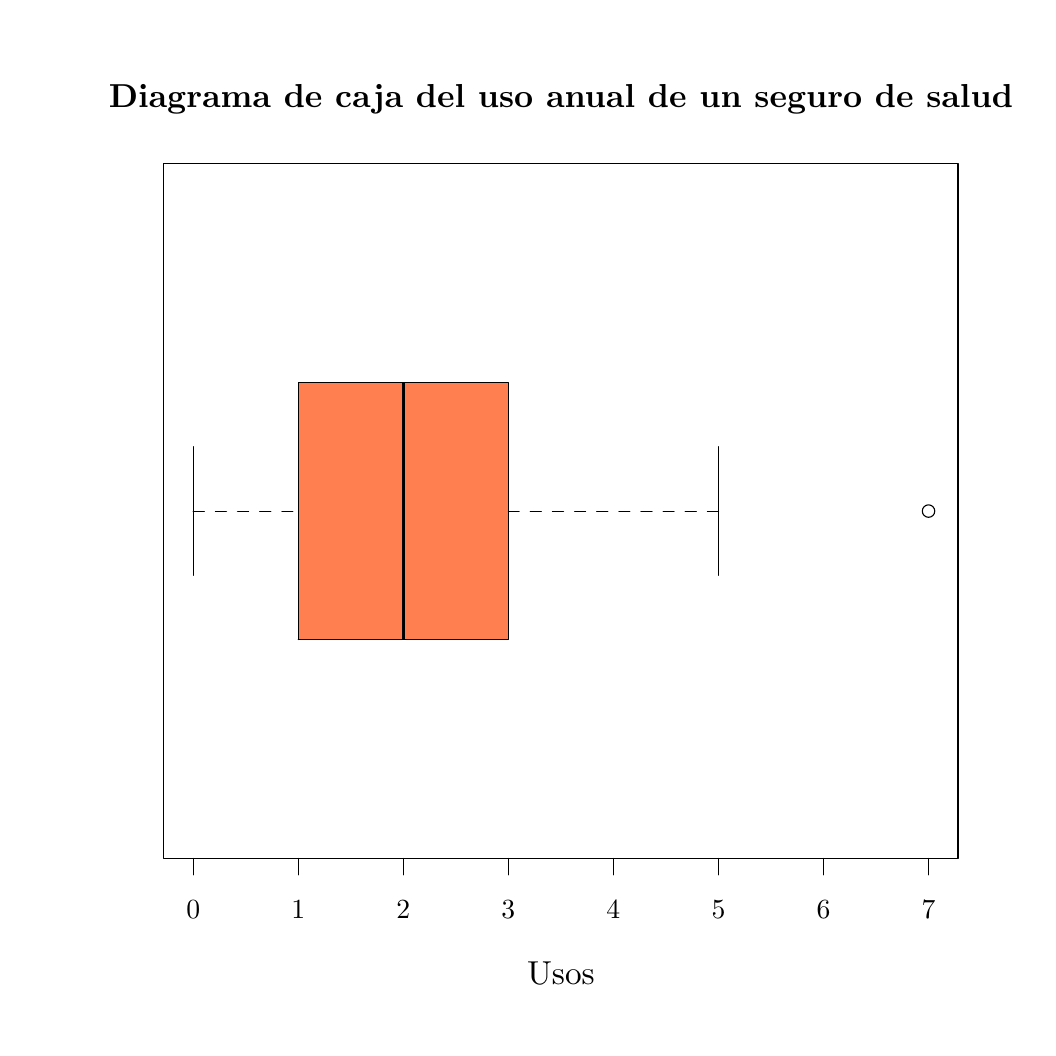
\begin{tikzpicture}[x=1pt,y=1pt]
\definecolor{fillColor}{RGB}{255,255,255}
\path[use as bounding box,fill=fillColor,fill opacity=0.00] (0,0) rectangle (361.35,361.35);
\begin{scope}
\path[clip] ( 49.20, 61.20) rectangle (336.15,312.15);
\definecolor{fillColor}{RGB}{255,127,80}

\path[fill=fillColor] ( 97.78,140.20) --
	( 97.78,233.15) --
	(173.70,233.15) --
	(173.70,140.20) --
	cycle;
\definecolor{drawColor}{RGB}{0,0,0}

\path[draw=drawColor,line width= 1.2pt,line join=round] (135.74,140.20) -- (135.74,233.15);

\path[draw=drawColor,line width= 0.4pt,dash pattern=on 4pt off 4pt ,line join=round,line cap=round] ( 59.83,186.67) -- ( 97.78,186.67);

\path[draw=drawColor,line width= 0.4pt,dash pattern=on 4pt off 4pt ,line join=round,line cap=round] (249.61,186.67) -- (173.70,186.67);

\path[draw=drawColor,line width= 0.4pt,line join=round,line cap=round] ( 59.83,163.44) -- ( 59.83,209.91);

\path[draw=drawColor,line width= 0.4pt,line join=round,line cap=round] (249.61,163.44) -- (249.61,209.91);

\path[draw=drawColor,line width= 0.4pt,line join=round,line cap=round] ( 97.78,140.20) --
	( 97.78,233.15) --
	(173.70,233.15) --
	(173.70,140.20) --
	( 97.78,140.20);

\path[draw=drawColor,line width= 0.4pt,line join=round,line cap=round] (325.52,186.67) circle (  2.25);
\end{scope}
\begin{scope}
\path[clip] (  0.00,  0.00) rectangle (361.35,361.35);
\definecolor{drawColor}{RGB}{0,0,0}

\path[draw=drawColor,line width= 0.4pt,line join=round,line cap=round] ( 59.83, 61.20) -- (325.52, 61.20);

\path[draw=drawColor,line width= 0.4pt,line join=round,line cap=round] ( 59.83, 61.20) -- ( 59.83, 55.20);

\path[draw=drawColor,line width= 0.4pt,line join=round,line cap=round] ( 97.78, 61.20) -- ( 97.78, 55.20);

\path[draw=drawColor,line width= 0.4pt,line join=round,line cap=round] (135.74, 61.20) -- (135.74, 55.20);

\path[draw=drawColor,line width= 0.4pt,line join=round,line cap=round] (173.70, 61.20) -- (173.70, 55.20);

\path[draw=drawColor,line width= 0.4pt,line join=round,line cap=round] (211.65, 61.20) -- (211.65, 55.20);

\path[draw=drawColor,line width= 0.4pt,line join=round,line cap=round] (249.61, 61.20) -- (249.61, 55.20);

\path[draw=drawColor,line width= 0.4pt,line join=round,line cap=round] (287.57, 61.20) -- (287.57, 55.20);

\path[draw=drawColor,line width= 0.4pt,line join=round,line cap=round] (325.52, 61.20) -- (325.52, 55.20);

\node[text=drawColor,anchor=base,inner sep=0pt, outer sep=0pt, scale=  1.00] at ( 59.83, 39.60) {0};

\node[text=drawColor,anchor=base,inner sep=0pt, outer sep=0pt, scale=  1.00] at ( 97.78, 39.60) {1};

\node[text=drawColor,anchor=base,inner sep=0pt, outer sep=0pt, scale=  1.00] at (135.74, 39.60) {2};

\node[text=drawColor,anchor=base,inner sep=0pt, outer sep=0pt, scale=  1.00] at (173.70, 39.60) {3};

\node[text=drawColor,anchor=base,inner sep=0pt, outer sep=0pt, scale=  1.00] at (211.65, 39.60) {4};

\node[text=drawColor,anchor=base,inner sep=0pt, outer sep=0pt, scale=  1.00] at (249.61, 39.60) {5};

\node[text=drawColor,anchor=base,inner sep=0pt, outer sep=0pt, scale=  1.00] at (287.57, 39.60) {6};

\node[text=drawColor,anchor=base,inner sep=0pt, outer sep=0pt, scale=  1.00] at (325.52, 39.60) {7};
\end{scope}
\begin{scope}
\path[clip] (  0.00,  0.00) rectangle (361.35,361.35);
\definecolor{drawColor}{RGB}{0,0,0}

\node[text=drawColor,anchor=base,inner sep=0pt, outer sep=0pt, scale=  1.20] at (192.68,332.61) {\bfseries Diagrama de caja del uso anual de un seguro de salud};

\node[text=drawColor,anchor=base,inner sep=0pt, outer sep=0pt, scale=  1.20] at (192.68, 15.60) {Usos};
\end{scope}
\begin{scope}
\path[clip] (  0.00,  0.00) rectangle (361.35,361.35);
\definecolor{drawColor}{RGB}{0,0,0}

\path[draw=drawColor,line width= 0.4pt,line join=round,line cap=round] ( 49.20, 61.20) --
	(336.15, 61.20) --
	(336.15,312.15) --
	( 49.20,312.15) --
	( 49.20, 61.20);
\end{scope}
\end{tikzpicture}
